\documentclass{article}
\usepackage{titrages}
\pgfplotsset{compat=1.18}
\titragedefinir{acetique}{volume = 10, becher = { espece = { pKa = 4.76, C = 0.1, lambda = {0, 4.09} } }, burette = { base forte = 0.1 }, volume max = 20}
\titragedefinir{phosphorique}{volume = 10, becher = { espece = { pKa = {2.15, 7.20, 12.35}, C = 0.1 } }, burette = { base forte = 0.1 }, volume max = 40}
\titragedefinir{ammoniac}{volume = 10, becher = { espece = { pKa = 9.25, C = 0.1, forme = 1, charge = 1, lambda = {7.35, 0} } }, burette = { acide fort = 0.1 }, volume max = 20}
\titragedefinir{fort}{volume = 100, becher = { acide fort = 0.01 }, burette = { base forte = 0.1 }, volume max = 20, conductivite corrigee = true}
\titragedefinir{faible}{volume = 20, becher = { acide fort = 0.05, espece = { pKa = 4.76, C = 0.05 } }, burette = { espece = { pKa = 9.25, C = 0.1, forme = 1 } }, volume max = 30}
\titrageredoxdefinir{cerium}{volume = 10, becher = { espece = { E0 = 0.77, C = 0.1 } }, burette = { espece = { E0 = 1.72, C = 0.1, forme = ox } }, reference = ECS, volume max = 20}
\titrageredoxdefinir{vanadium}{volume = 10, becher = { espece = { E0 = {-0.26, 0.34, 1.00}, n = {1, 1, 1}, H = {0, 2, 2}, C = 0.1 } }, burette = { espece = { E0 = 1.51, n = 5, H = 8, C = 0.02, forme = ox } }, pH = 0, volume max = 40}
\begin{document}
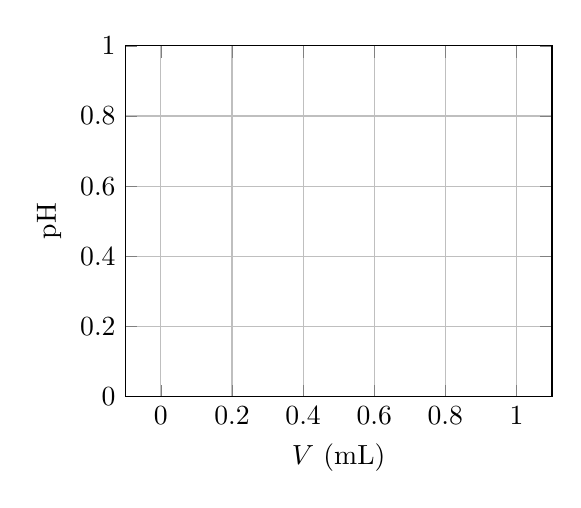
\begin{tikzpicture}
\begin{axis}[xlabel={$V$ (mL)}, ylabel=pH, ymin=0, ymax=14, grid=both, width=7cm]
  \addplottitrage[thick]{acetique}
  \addplottitrage[thick]{phosphorique}
  \addplottitrage[thick]{ammoniac}
  \addplottitrage[thick]{faible}
\end{axis}
\end{tikzpicture}
\begin{tikzpicture}
\begin{axis}[xlabel={$V$ (mL)}, ylabel={$\sigma$ (mS/cm)}, width=7cm]
  \addplottitrageconductivite[thick]{acetique}
  \addplottitrageconductivite[thick]{fort}
  \addplottitrageconductivite[thick]{ammoniac}
\end{axis}
\end{tikzpicture}

\titragesreglages{E min = -0.5, E max = 1.8}
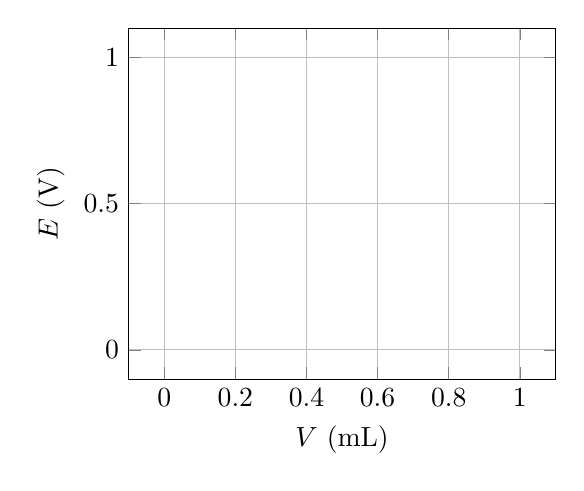
\begin{tikzpicture}
\begin{axis}[xlabel={$V$ (mL)}, ylabel={$E$ (V)}, width=7cm, grid=both]
  \addplottitrage[thick]{cerium}
  \addplottitrage[thick]{vanadium}
\end{axis}
\end{tikzpicture}
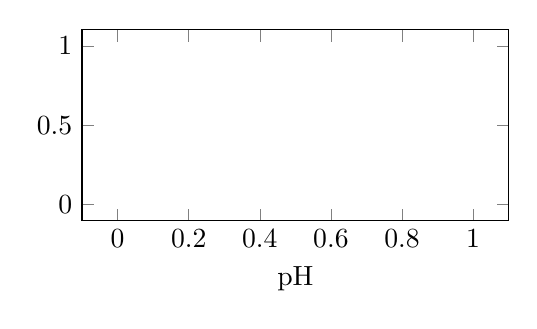
\begin{tikzpicture}
\begin{axis}[xlabel=pH, width=7cm, height=4cm]
  \addplotfractions[thick]{2.15, 7.20, 12.35}
\end{axis}
\end{tikzpicture}
\end{document}
